\documentclass[a4paper]{article}

\usepackage{graphicx}
\usepackage{multicol}
\usepackage{amsmath}
\usepackage{booktabs}
\usepackage[left=1cm, right=1.5cm, top=1.5cm, bottom=1.2cm]{geometry}

\begin{document}

\section{Combinatorics}
\begin{center}
\begin{tabular}{@{}ll|ll@{}}
\toprule
\multicolumn{4}{c}{Classical Problems} \\ \midrule
HanoiTower(HT) min steps 	&	$T_n = 2^n - 1$	&	Regions by $n$ lines & $L_n = n(n+1)/2+1$ \\
Regions by $n$ Zig lines	&	$Z_n=2n^2-n+1$	&	Joseph Problem (every $m$-th)	&	$F_1=0$, $F_i=(F_{i-1}+m)\% i $\\ 
Joseph Problem (every $2$nd)	&	rotate $n$ $1$-bit to left	&	HanoiTower (no direct $A$ to $C$) 	&	$T_n = 3^n - 1$ \\ 
Bounded regions by $n$ lines	&	$(n^2-3n+2)/2$	&	Joseph given pos $j$,find $m$.($\downarrow$con.)	& $m\equiv 1$ (mod $\frac{L}{p})$,\\
HT min steps A to C clockw.& $Q_n=2R_{n-1}+1$ &  $L(n)=lcm(1,...,n)$, $p$ prime $\in [\frac{n}{2},n]$ & $m\equiv j+1-n$ (mod $p$)\\
HT min steps C to A clockw.& $R_n=2R_{n-1}+Q_{n-1}+2$ & $\sum_{i=1}^n i^2 = n(n+1)(2n+1)/6$ & $\sum_{i=1}^n i^3 = n^2(n+1)^2/4$\\
Egyptian Fraction & $\frac{m}{n}=\frac{1}{\lceil n/m \rceil}+(\frac{m}{n}-\frac{1}{\lceil n/m \rceil})$ & Farey Seq given $m/n$, $m'/n'$ & $m''=\lfloor (n+N)/n' \rfloor m'-m$\\
Farey Seq given $m/n$, $m''/n''$ & $m'/n'=\frac{m+m''}{n+n''}$ & $m/n=0/1$, $m'/n'=1/N$ & $n''=\lfloor (n+N)/n' \rfloor n'-n$\\
\#labeled rooted trees & $n^{n-1}$ & \#labeled unrooted trees & $n^{n-2}$ \\
\#SpanningTree of $G$ (no SL) & $C(G)=D(G)-A(G)(\downarrow)$ & Stirling's Formula & $n! \sim \sqrt{2 \pi n} \left(\frac{n}{e}\right)^n(1+\frac{1}{12n})$ \\
$D:$ DegMat; $A:$ AdjMat & $Ans=|\det(C-1r-1c)|$ & Farey Seq & $m n' - m' n = -1$ \\
& &\#ways $0\rightarrow m$ in $n$ steps (never $<0$) &  $\frac{m+1}{\tfrac{n+m}2+1}\binom{n}{\tfrac{n+m}2}$ \\
\multicolumn{3}{l}{$\#seq\langle a_0,...,a_{mn} \rangle$ of $1$'s and $(1-m)$'s with sum $+1 = \binom{mn+1}{n}\frac{1}{mn+1}=\binom{mn}{n}\frac{1}{(m-1)n+1}$ } \\

\bottomrule
\end{tabular}
\end{center}

\begin{center}
\begin{tabular}{@{}l|l|l@{}}
\toprule
\multicolumn{3}{c}{Binomial Coefficients} \\ \midrule
$\binom{n}{k}=\frac{n!}{k!(n-k)!}$, int $n \ge k \ge 0$ & $\binom{n}{k}=\binom{n}{n-k}$, int $n\ge 0$, int $k$ & $\binom{r}{k}=\frac{r}{k}\binom{r-1}{k-1}$, int $k\ne 0$ \\
$\binom{r}{k}=(-1)^k \binom{k-r-1}{k}$, int $k$ & $\binom{r}{m}\binom{m}{k}=\binom{r}{k}\binom{r-k}{m-k}$, int $m,k$ & $(x+y)^r = \sum_{k} \binom{r}{k}x^ky^{r-k}$, int $r \ge 0$ or $|x/y|<1$ \\
$\binom{r}{k}=\binom{r-1}{k}+\binom{r-1}{k-1}$, int $k$ & $\sum_{k\le n}\binom{r+k}{k}=\binom{r+n+1}{n}$, int $n$ & $\sum_{k=0}^n\binom{k}{m}=\binom{n+1}{m+1}$, int $m,n\ge 0$ \\
$\binom{r+s}{n}=\sum_{k}\binom{r}{k}\binom{s}{n-k}$, int $n$ & $\sum_{k\le m}\binom{r}{k}(\frac{r}{2}-k)=\frac{m+1}{2}\binom{r}{m+1}$, int $m$ & $\sum_{k\le m}\binom{r}{k}(-1)^k = (-1)^m\binom{r-1}{m}$, int $m$ \\
$\sum_{k}\binom{r}{m+k}\binom{s}{n-k}=\binom{r+s}{m+n}$, int $m,n$ & $\binom{\binom{k}{2}}{2}=3\binom{k+1}{4}$ \quad \vline \quad $\sum_{i=0}^n\binom{n}{i}^2=\binom{2n}{n}$ & $\sum_{k}\binom{l}{m+k}\binom{s}{n+k}=\binom{l+s}{l-m+n}$ int $l\ge0$, int $m,n$\\
$\sum_k\binom{n}{2k}=2^{n-even(n)}$ & $lcm_{i=0}^n\binom{n}{i}=\frac{L(n+1)}{n+1}$ & $S(n,1)=S(n,n)=n \Rightarrow S(n,k)=\binom{n+1}{k}-\binom{n-1}{k-1}$\\
$\sum_{i=1}^n\binom{n}{i}F_i=F_{2n}$, $F_n=$ $n$-th Fib & $\sum_i\binom{n-i}{i}=F_{n+1}$ & \\

\bottomrule
\end{tabular}
\end{center}

\begin{center}
\begin{tabular}{@{}l|l|l@{}}
\toprule
\multicolumn{3}{c}{Famous Numbers} \\ \midrule

Catalan	&	$C_0=1$, $C_n=\frac{1}{n+1}\binom{2n}{n} = \sum_{i=0}^{n-1}C_iC_{n-i-1} = \frac{4n-2}{n+1}C_{n-1}$  & \\
Stirling 1st kind & $\left[{0\atop 0}\right]=1$, $\left[{n\atop 0}\right]=\left[{0\atop n}\right]=0$, $\left[{n\atop k}\right]=(n-1)\left[{n-1\atop k}\right]+\left[{n-1\atop k-1}\right]$ & \#perms of $n$ objs with exactly $k$ cycles\\
Stirling 2nd kind & $\left\{{n\atop 1}\right\}=\left\{{n\atop n}\right\}=1$, $\left\{{n\atop k}\right\} = k \left\{{ n-1 \atop k }\right\} + \left\{{n-1\atop k-1}\right\}$ & \#ways to partition $n$ objs into $k$ nonempty sets\\
Euler	& $\left \langle {n\atop 0} \right \rangle = \left \langle {n\atop n-1} \right \rangle = 1 $, $\left \langle {n\atop k} \right \rangle = (k+1) \left \langle {n-1\atop {k}} \right \rangle + (n-k)\left \langle {{n-1}\atop {k-1}} \right \rangle$ & \#perms of $n$ objs with exactly $k$ ascents \\
Euler 2nd Order &  $\left \langle \!\!\left \langle {n\atop k} \right \rangle \!\! \right \rangle = (k+1) \left \langle \!\! \left \langle {{n-1}\atop {k}} \right \rangle \!\! \right \rangle +(2n-k-1)\left \langle \!\! \left \langle {{n-1}\atop {k-1}} \right \rangle  \!\! \right \rangle$ & \#perms of ${1,1,2,2,...,n,n}$ with exactly $k$ ascents \\

\bottomrule
\end{tabular}
\end{center}


{\bf Burnside's Lemma:} $L=\frac{1}{|G|}\sum_{k=1}^n|Z_k|=\frac{1}{|G|}\sum_{a_i \in G}C_1(a_i)$. $Z_k:$ the set of permutations in $G$ under which $k$ stays stable;  $C_1(a_i):$ the number of cycles of order $1$ in $a_i$. \quad {\bf P\'olya's Theorem:} The number of colorings of $n$ objects with $m$ colors $L=\frac{1}{|\overline{G}|}\sum_{g_i \in \overline{G}}{m^{c(g_i)}}$. $\overline{G}:$ the group over $n$ objects;  $c(g_i):$the number of cycles in $g_i$.

% Regular Polyhedron Coloring
\begin{center}
\begin{tabular}{@{}ll|lr@{}}
\toprule
\multicolumn{4}{c}{Regular Polyhedron Coloring {\bf with at most $n$ colors (up to isomorph)} } \\ \hline
\it Description		&	\it Formula	 & Remarks & \\ \hline
 {\bf vertices of octahedron} or {\bf faces of cube} 	&	$ (n^6 + 3 n^4 + 12 n^3 + 8 n^2)/24$  & & $(V,F,E)$\\ 

{\bf vertices of cube} or {\bf faces of octahedron}	&	$ (n^8 + 17 n^4 + 6 n^2)/24$  &	tetrahedron: & $(4,4,6)$ \\

{\bf edges of cube} or {\bf edges of octahedron}		&	$ (n^{12} + 6 n^7 + 3 n^6 + 8 n^4 + 6 n^3)/24$   & cube: & $(8,6,12)$ \\

{\bf vertices} or {\bf faces of tetrahedron}			&	$(n^4 + 11 n^2)/12$ 	& octahedron:& $(6,8,12)$ \\

{\bf edges of tetrahedron}	&	$(n^6 + 3 n^4 + 8 n^2)/12$ & dodecahedron: & $(20,12,30)$ \\

{\bf vertices of icosahedron} or {\bf faces of dodecahedron} & $(n^{12} + 15 n^6 + 44 n^4)/60$ & icosahedron & $(12,20,30)$\\

{\bf vertices of dodecahedron} or {\bf faces of icosahedron} & $(n^{20} + 15 n^{10} + 20 n^8 + 24 n^4)/60$ &\\

{\bf edges of dodecahedron} or {\bf edges of icosahedron} & $(n^{30} + 15 n^{16} + 20 n^{10} + 24 n^6)/60$ & \multicolumn{2}{c}{\emph{This row may be wrong.}}\\

\bottomrule
\end{tabular}
\end{center}
\newpage
\section{Number Theory}
\begin{center}
\begin{tabular}{@{}l|l|l@{}}
\toprule
\multicolumn{3}{c}{Classical Theorems} \\ \midrule
exp of $p$ in $n!$ is $\sum_{i\ge 1}[\frac{n}{p^i}]$  & $p_n \sim n\log n$; \quad $\forall_{n>1} \exists_{n<p<2n}: p$ is prime &  $\pi(x) \sim \frac{x}{\log x}$; \quad Norm$(\alpha\beta)=$ Norm$(\alpha)\cdot$Norm$(\beta)$\\
lcm$(a,b)$=$\frac{ab}{\gcd(a,b)}$ & $a\equiv b$ $($mod $x,y)\Rightarrow a\equiv b$ $($mod lcm$(x,y))$ & All prime factors of $2^{2^n}+1$ have form $2^{n+2}k+1$\\
$(2^a-1, 2^b-1)=2^{(a,b)}-1$ &  $ac\equiv bc$ $($mod $m)\Rightarrow a\equiv b ($mod $\frac{m}{\gcd(c,m)})$ & $n$-plygn drawable $\Leftrightarrow n=2^k\prod F_i$, $F_i$ fermatNum  \\
$p_i$ is prime, $\prod_{p_i\le n}p_i<4^n$  & \multicolumn{2}{l}{$W\equiv d+[2.6m-0.2]-2C+Y+\left[\frac{Y}{4}\right]+\left[\frac{C}{4}\right] (\%7)$. \quad$m=11,12,1$ for Ja,Fe,Ma. J\&F$\in$lastyear}  \\
\bottomrule
\end{tabular}
\end{center}


\begin{center}
\begin{tabular}{@{}l|l|l@{}}
\toprule
\multicolumn{3}{c}{Classical Theorems} \\ \midrule
$p$ prime $\Leftrightarrow (p-1)!\equiv -1 (\%p)$  &  $a\perp m \Rightarrow a^{\phi(m)}=1 (\%m)$  & Min general idx $\lambda(n)$: $\forall_a:a^{\lambda(n)}\equiv 1(\%n)$ \\
$\sum_{d|n}\phi(d)=\sum_{d|n}\phi(n/d)=n$ & $\sum_{m\perp n,m<n}m=\frac{n\phi(n)}{2}$ & $\sum_{i=1}^n\sigma_0(i) = 2\sum_{i=1}^{[\sqrt{n}]}[n/j]-[\sqrt{n}]^2$\\
$(\sum_{d|n}\sigma_0(d))^2=\sum_{d|n}\sigma_0(d)^3$ & $\sum_{d|n}n\sigma_1(d)/d = \sum_{d|n}d\sigma_0(d)$ & $[\sqrt{n}]$  Newton: $y=[\frac{x+[n/x]}{2}]$, $x_0=2^{[\frac{\log_2(n)+2}{2}]}$ \\
$\sigma_0(p_1^{e_1}\cdots p_s^{e_s})=\prod_{i=1}^s(e_i+1)$ & $\sigma_1(p_1^{e_1}\cdots p_s^{e_s})=\prod_{i=1}^s \frac{p_i^{e_i+1}-1}{p_i-1}$ & $r_1=4$, $r_k\equiv r_{k-1}^2-2(\%M_p)$, $M_p$ prime $\Leftrightarrow r_{p-1}\equiv 0(\%M_p)$\\
$\mu(p_1p_2\cdots p_s)=(-1)^s$, else $0$ & $\sum_{d|n}\mu(d)=1$ if $n=1$, else $0$ & $F(n)=\sum_{d|n}f(d)\Leftrightarrow f(n)=\sum_{d|n}\mu(d)F(\frac{n}{d})$\\
$n=\sum_{d|n}\mu(\frac{n}{d})\sigma_1(d)$  & $n=2,4,p^t,2p^t\Leftrightarrow n$ has p\_roots & $a\perp n$, then $a^i\equiv a^j(\%n)\Leftrightarrow i\equiv j (\% $ord$_n(a))$ \\
$1=\sum_{d|n}\mu(\frac{n}{d})\sigma_0(d)$  & $r=$ ord$_n(a)$, ord$_n(a^u)= \frac{r}{\gcd(r,u)}$ & $r$ p\_root of $n$, then $r^u$ is p\_root of $n \Leftrightarrow u\perp\phi(n)$ \\
ord$_n(a)=$ ord$_n(a^{-1})$ & $r$ p\_root of $n\Leftrightarrow r^{-1}$ p\_root of $n$  & $n$ has p\_roots $\Leftrightarrow n$ has $\phi(\phi(n))$ p\_roots \\
$a^n \equiv a^{\phi(m)+n\%\phi(m)} (\%m)$ & \multicolumn{2}{l}{$\lambda(2^t)=2^{t-2}$, $\lambda(p^t)=\phi(p^t)=(p-1)p^{t-1}$, $\lambda(2^{t_0}p_1^{t_1}\cdots p_m^{t_m})=lcm(\lambda(2^{t0}),\phi(p_1^{t_1}),\cdots,\phi(p_m^{t_m}))$} \\
$\left(\frac{a}{p}\right)\equiv a^{(p-1)/2} (\%p)$ & \multicolumn{2}{l}{Legendre sym $\left(\frac{a}{p}\right)=1$ if $a$ is quad residue $\%p$; $-1$ if $a$ is non-residue; $0$ if $a=0$} \\ \
$a\equiv b (\%p) \Rightarrow \left(\frac{a}{p}\right) = \left(\frac{b}{p}\right)$ & $ \left(\frac{a}{p}\right) \left(\frac{b}{p}\right)= \left(\frac{ab}{p}\right)$;  $ \left(\frac{a^2}{p}\right)=1$ &  $a \perp p$, $s$ from $a,2a,...,\frac{p-1}{2}a (\%p)$ are $>\frac{p}{2} \Rightarrow \left(\frac{a}{p}\right)=(-1)^s$\\
$ \left(\frac{p}{q}\right)\left(\frac{q}{p}\right)=(-1)^{\frac{p-1}{2}\frac{q-1}{2}} $  &  \multicolumn{2}{l}{Gauss Integer $\pi=a+bi$. Norm$(\pi)=p$ prime $\Rightarrow$ $\pi$ and $\overline\pi$ prime, $p$ not prime}\\

\bottomrule
\end{tabular}
\end{center}


\section{Probability}
\begin{center}
\begin{tabular}{@{}ll|ll@{}}
\toprule
\multicolumn{4}{c}{Classical Formulae} \\ \midrule
Ballot.Always $\#A > k\#B$ & $Pr=\frac{a-kb}{a+b}\binom{a+b}{a}$ &  Ballot.Always $\#B-\#A\le k$ & $Pr=1-\frac{n!m!}{(n+k+1)!(m-k-1)!}$  \\
$E(X+Y)=EX+EY$ & $E(\alpha X)=\alpha EX$ & if X,Y indep. $\Leftrightarrow E(XY)=(EX)(EY)$
\\

\bottomrule
\end{tabular}
\end{center}

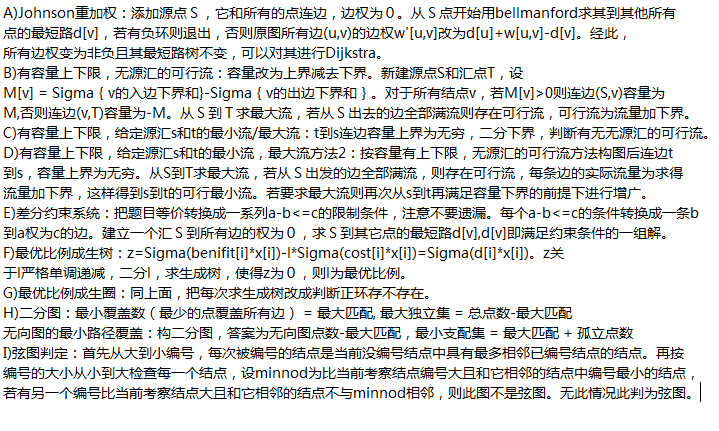
\includegraphics{chinese.png}




\end{document}